\Chapter{Optimalizálás}

\section{Profilozás}
Azoknál a módszereknél, amelyek mért futásidejében jelentős különbség adódott a C-s, illetve a Rustos implementáció között van egy közös jellemzőjük: nagyméretű inputot olvasnak be fájlból. Így adódik a felvetés, hogy a fájl beolvasáshoz szükséges idő jelenti a differenciát a két implementáció között.

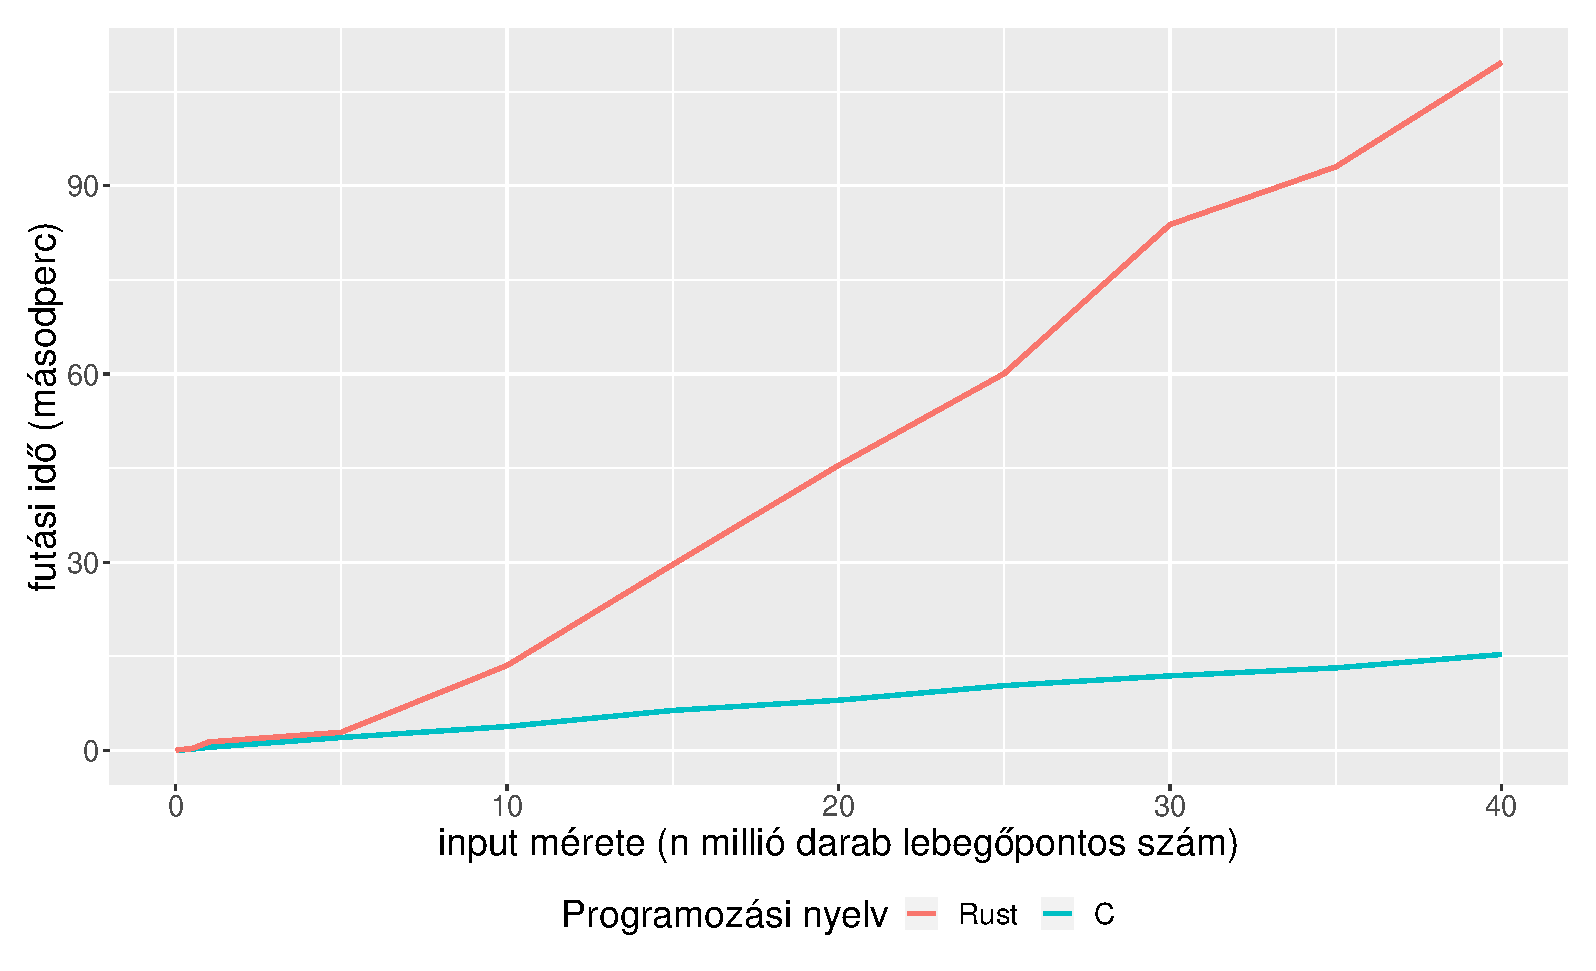
\includegraphics[width=15.5cm]{kepek/file_read.eps}
A grafikonon látható, hogy Rustban a beolvasás jóval lassabb, a futásidők különbségét magyarázza.
\subsection{Futásidők a fájl beolvasása nélkül}
\subsubsection{Kupacrendezés}
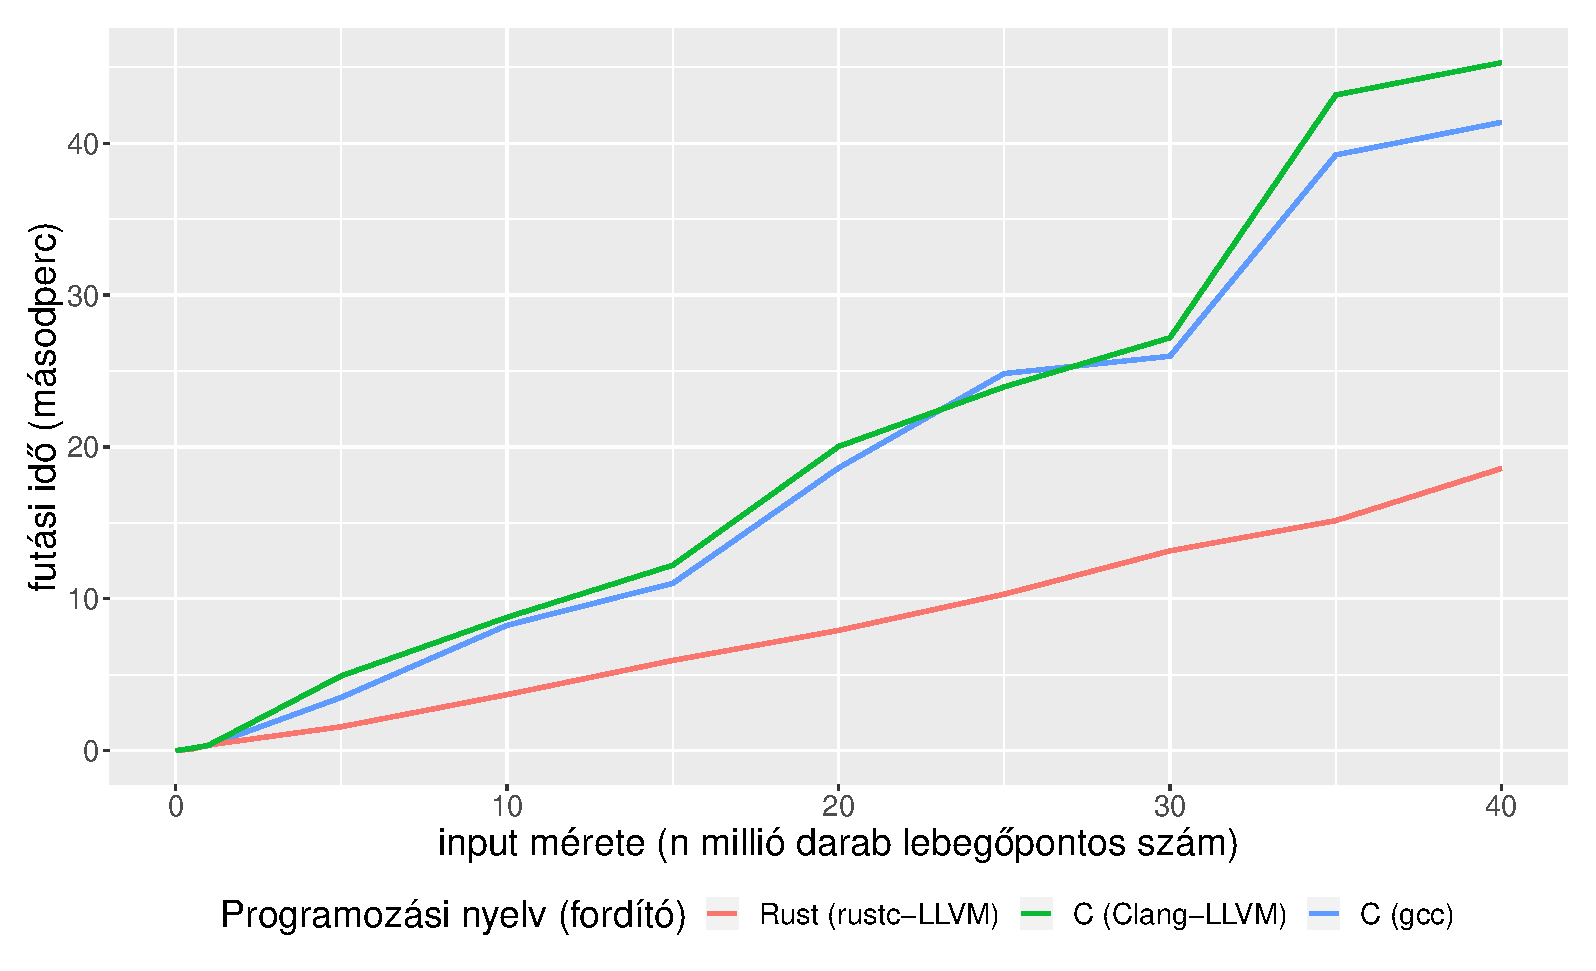
\includegraphics[width=15.5cm]{kepek/heap_sort_run_without_read.eps}
\subsubsection{Shell-rendezés}
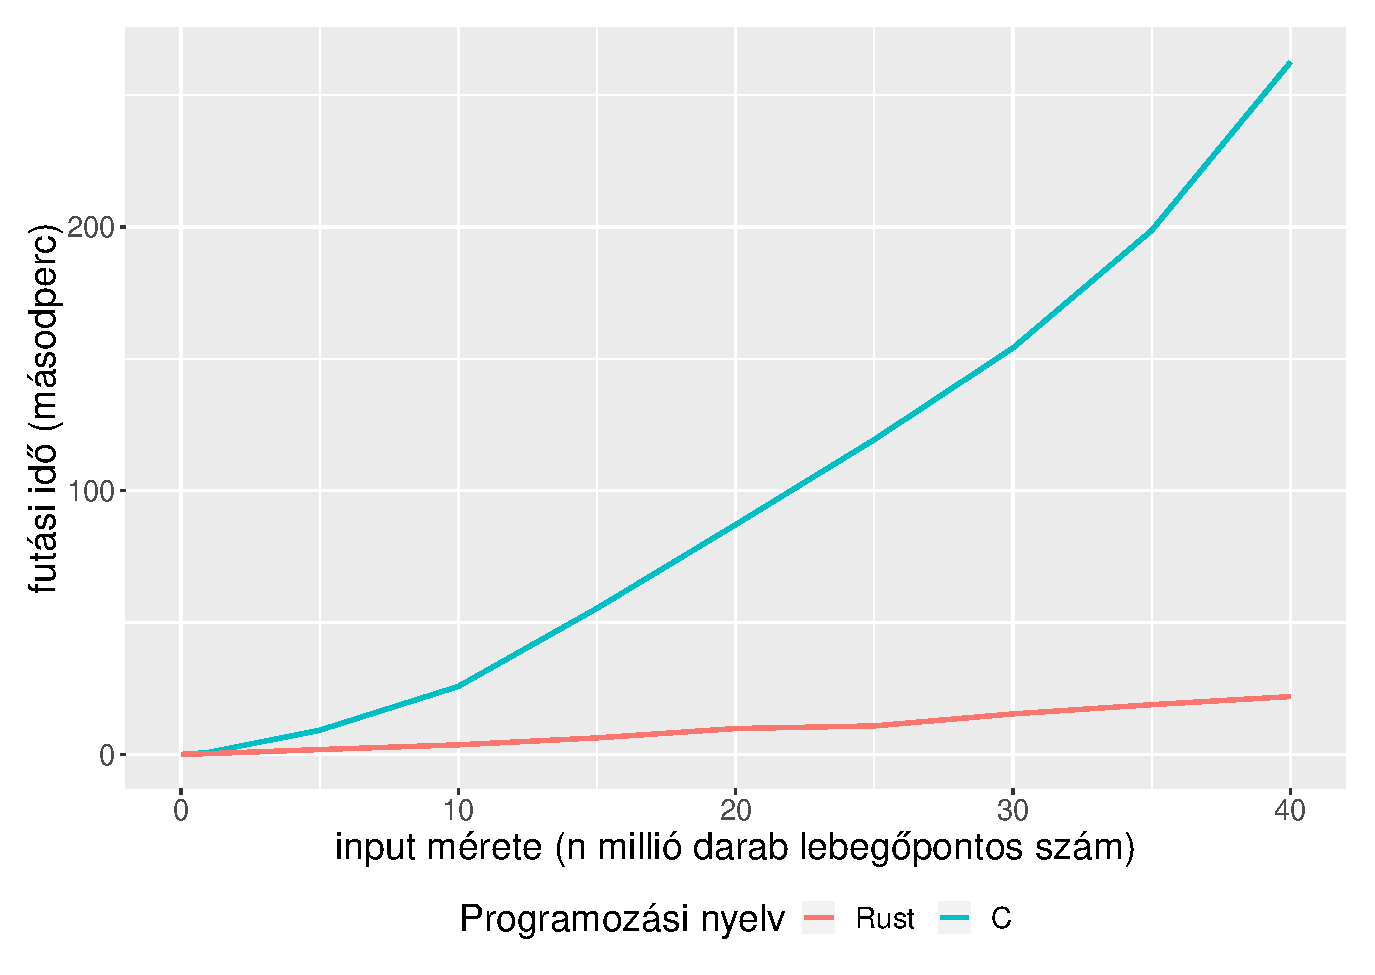
\includegraphics[width=15.5cm]{kepek/shells_sort_run_without_read.eps}
\subsubsection{Gyorsrendezés}
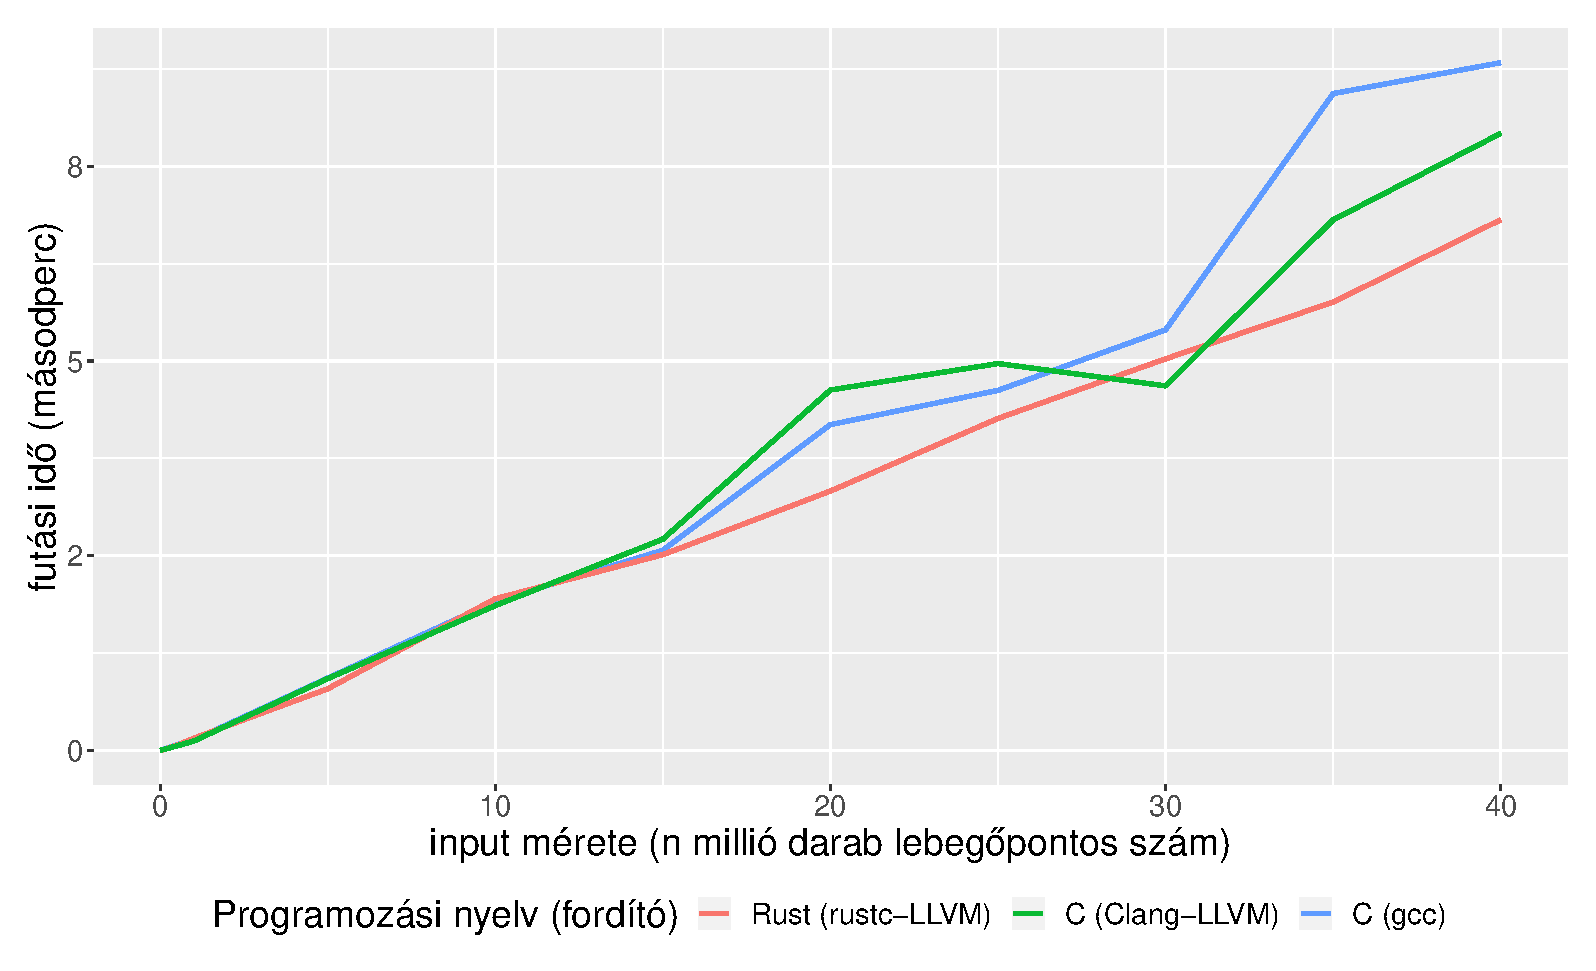
\includegraphics[width=15.5cm]{kepek/quicksort_run_without_read.eps}
\subsubsection{Lineáris interpoláció}
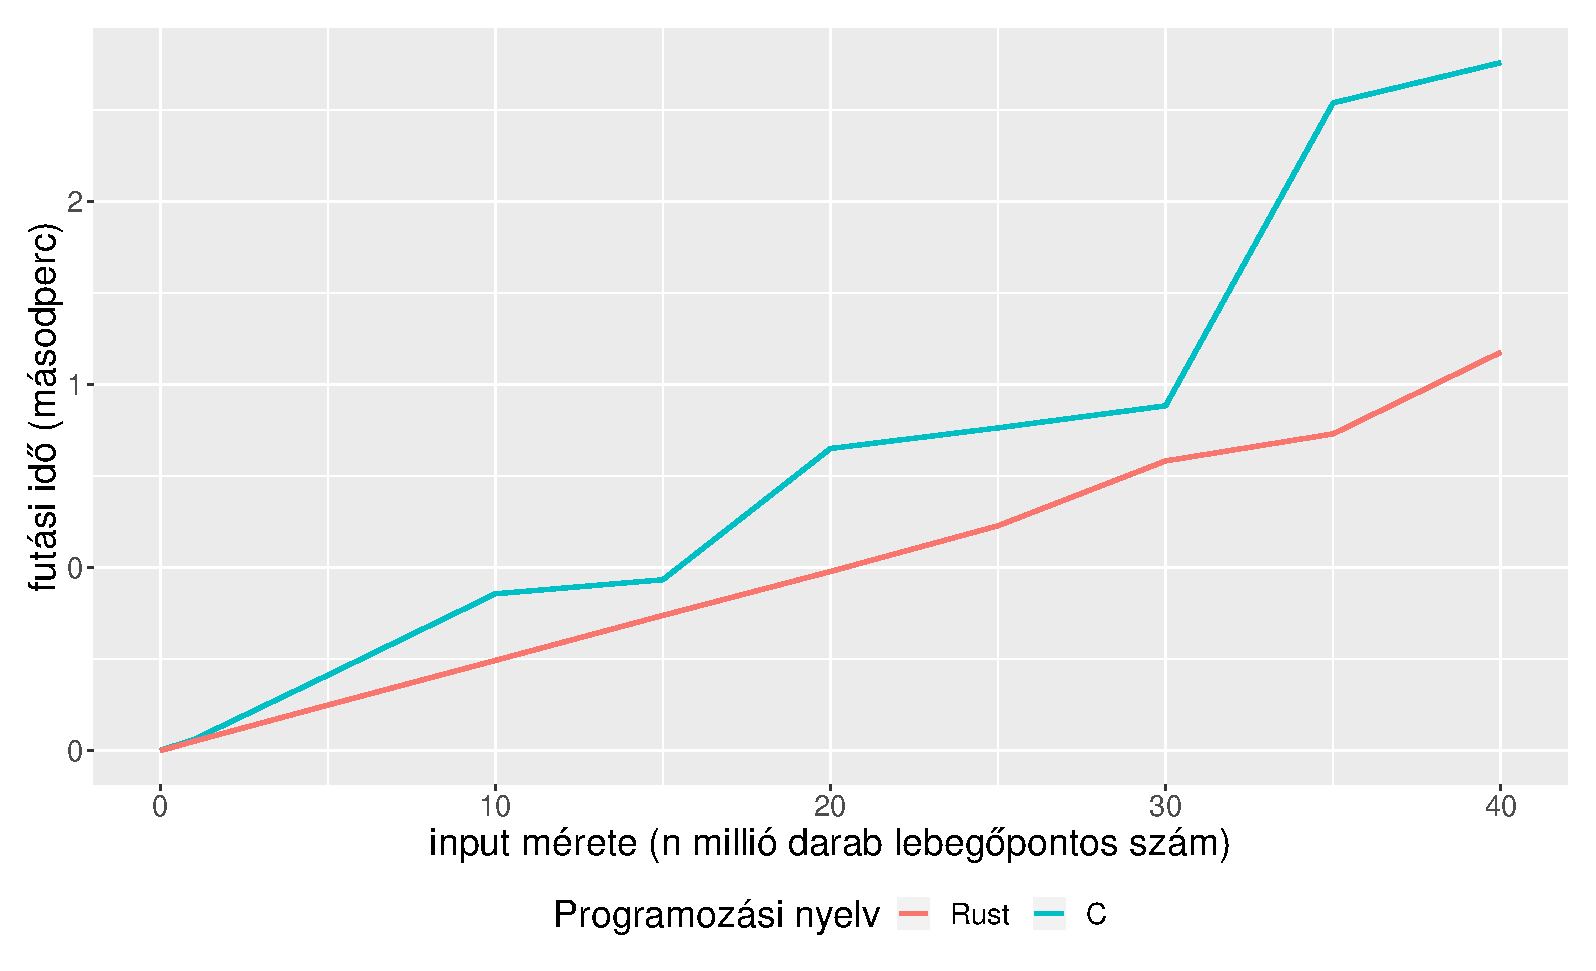
\includegraphics[width=15.5cm]{kepek/linear_interpolation_run_without_read.eps}
Látható, hogy maga a módszer a Rust implementációban minden esetben gyorsabb, ha az inputfájlok beolvasását nem mérjük.

\section{Technikai részletek}
Lebegőpontos számok ábrázolását a Rust az IEEE-754-es szabványnak megfelelően végzi. Az egyszeres pontosságú lebegőpontos számokat az \lstinline{f32}, a dupla pontosságú lebegőpontos számokat pedig az \lstinline{f64} típusok szolgáltatják. C-ben ez nincs specifikálva, de általában az IEEE szabványát követi. Az egyszeres pontosságú a \lstinline{float}, a dupla pontosságú lebegőpontos szám a \lstinline{double} típussal reprezentálható.
%https://doc.rust-lang.org/book/ch03-02-data-types.html

A Rust nyelven implementált rendezési eljárások esetén a beépített \lstinline{Vec} adatszerkezetet használtam, melynek működéséhez hasonló saját típust definiáltam C-ben is. Ugyanakkor megemlítendő, hogy a C-s \lstinline{Vec} típus nem implementálja a Rustban meglévő vektor típus által implementált összes metódust, csak azt azokat, amelyek a dolgozatban bemutatott módszerek által használtak.
%https://doc.rust-lang.org/stable/nomicon/vec-alloc.html
\cppstyle{\begin{lstlisting}[language=c++]
typedef struct Vec {
  float *elements;
  size_t len;
  size_t capacity;
}

void vec_init(Vec *vec, size_t with_capacity) {
    vec->elements = (float*)malloc(with_capacity * sizeof(float) );
    vec->len = 0;
    vec->capacity = with_capacity;
}

void vec_insert(Vec *vec, float element) {
    if (vec->len == vec->capacity) {
        vec->capacity *= 2;
        vec->elements = (float *)realloc(vec->elements, vec->capacity * sizeof(float) );
    }
    vec->elements[vec->len++] = element;
}

Vec vec_copy(Vec *original_vec) {
    Vec new_vec;
    vec_init(&new_vec, original_vec->capacity);
    
    for (unsigned i = 0; i < original_vec->len; i++) {
        vec_insert(&new_vec, original_vec->elements[i]);
    }
    return new_vec;
}

void vec_free(Vec *vec) {
    free(vec->elements);
    vec->elements = NULL;
    vec->len = vec->capacity = 0;
}
\end{lstlisting}}

\section{Fordítóprogram-specifikus beállítások}
\subsection{A GNU GCC fordítóprogram specifikus beállításai (C)}
A C nyelvű implementációk fordításához a GNU GCC fordítóprogramot használtam, ami többféle optimalizálási lehetőséget is kínál. Alapértelmezetten, bármilyen opció megadása nélkül a fordító a fordítási időt próbálja minimalizálni.
\begin{itemize}
  \item Az \lstinline{-O1} opció bekapcsolja az összes olyan flaget, ami csökkentheti a kód méretét és a futási időt, anélkül, hogy a fordítási időt nagyban növelő opciót használna.
  \item Az \lstinline{-O2} opció bekapcsolja közel az összes olyan támogatott optimalizálási megoldást, ami nem jár együtt kompromisszumokkal a tárigény és a futási idő között. Tovább növeli a teljesítményt, viszont a fordítási idő is növekedhet az opció használatával.
  \item Az \lstinline{-O3} opció használ minden optimalizálást, amit az \lstinline{-O2} opció is, és még néhányat azon felül.
  \item Az \lstinline{-Ofast} opció futási sebességre optimalizál, használ minden optimalizálást, amit az \lstinline{-O3} kapcsoló is, ezeken felül pedig olyan optimalizálásokat is engedélyez, amelyek nem érvények minden szabványos programnak.
  \item Az \lstinline{-Os} opció a bináris méretére optimalizál. Használ minden optimalizálást, amit az \lstinline{-O2} opció is, kivéve azokat, amelyek sok esetben együtt járnak a tárigény növekedésével. Engedélyezi az \lstinline{-finline-funcions} kapcsolót, amely a fordítót a futási idő helyett a kódméret csökkentésére állítja. 
\end{itemize}
% https://gcc.gnu.org/onlinedocs/gcc/Optimize-Options.html
\subsection{A rustc fordítóprogram specifikus beállításai (Rust)}
\begin{itemize}
  \item A \lstinline{-C} vagy \lstinline{--codegen OPT[=VALUE]} opció használata esetén az \lstinline{opt-level} kapcsolóval állítható a fordító által alkalmazott optimalizálás szintje. A szint egyrészt 0-3 közötti egész szám lehet, ahol a 3 jelenti a leginkább optimalizált kimenetet. Az \lstinline{s} és \lstinline{z} szintek a fordítás során létrejövő bináris méretére optimalizál.
  \item Az \lstinline{-O} opció ekvivalens a \lstinline{-C opt-level=2} használatával.
\end{itemize}
